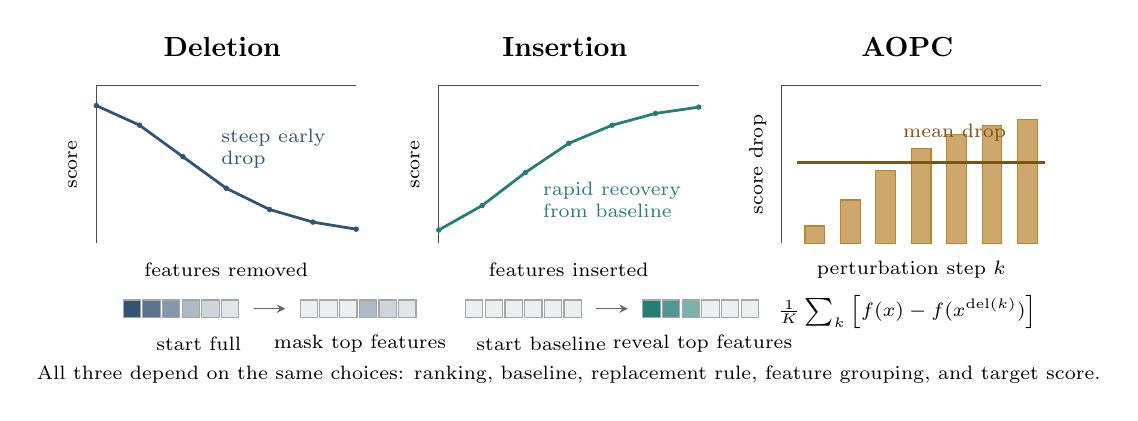
\begin{tikzpicture}[x=1cm,y=1cm,>=stealth]
\tikzset{
  panel/.style={draw=black!40, rounded corners=1pt},
  axis/.style={draw=black!70, line width=.35pt},
  feature/.style={draw=black!35, minimum width=.22cm, minimum height=.22cm, inner sep=0pt},
  note/.style={font=\scriptsize, align=left}
}

\definecolor{metricblue}{RGB}{50,83,116}
\definecolor{metricteal}{RGB}{38,125,117}
\definecolor{metricgold}{RGB}{178,119,28}
\definecolor{maskgray}{RGB}{236,239,241}

\begin{scope}[shift={(0,0)}]
  \node[font=\bfseries] at (1.85,2.95) {Deletion};
  \draw[axis] (.25,.45) -- (.25,2.45) -- (3.55,2.45);
  \node[font=\scriptsize,rotate=90] at (-.05,1.45) {score};
  \node[font=\scriptsize] at (1.9,.12) {features removed};
  \draw[metricblue,line width=1pt]
    (.25,2.2) -- (.8,1.95) -- (1.35,1.55) -- (1.9,1.15) -- (2.45,.88) -- (3.0,.72) -- (3.55,.63);
  \foreach \x/\y in {.25/2.2,.8/1.95,1.35/1.55,1.9/1.15,2.45/.88,3.0/.72,3.55/.63}
    \fill[metricblue] (\x,\y) circle (.035);
  \node[note,metricblue] at (2.5,1.65) {steep early\\drop};

  \foreach \i/\c in {0/metricblue!100,1/metricblue!80,2/metricblue!60,3/metricblue!40,4/metricblue!25,5/metricblue!15}
    \node[feature,fill=\c] at (.7+.25*\i,-.38) {};
  \draw[->,black!60] (2.25,-.38) -- (2.65,-.38);
  \foreach \i/\c in {0/maskgray,1/maskgray,2/maskgray,3/metricblue!40,4/metricblue!25,5/metricblue!15}
    \node[feature,fill=\c] at (2.95+.25*\i,-.38) {};
  \node[note] at (1.55,-.82) {start full};
  \node[note] at (3.6,-.82) {mask top features};
\end{scope}

\begin{scope}[shift={(4.35,0)}]
  \node[font=\bfseries] at (1.85,2.95) {Insertion};
  \draw[axis] (.25,.45) -- (.25,2.45) -- (3.55,2.45);
  \node[font=\scriptsize,rotate=90] at (-.05,1.45) {score};
  \node[font=\scriptsize] at (1.9,.12) {features inserted};
  \draw[metricteal,line width=1pt]
    (.25,.62) -- (.8,.93) -- (1.35,1.35) -- (1.9,1.72) -- (2.45,1.95) -- (3.0,2.1) -- (3.55,2.18);
  \foreach \x/\y in {.25/.62,.8/.93,1.35/1.35,1.9/1.72,2.45/1.95,3.0/2.1,3.55/2.18}
    \fill[metricteal] (\x,\y) circle (.035);
  \node[note,metricteal] at (2.45,1.0) {rapid recovery\\from baseline};

  \foreach \i in {0,...,5}
    \node[feature,fill=maskgray] at (.7+.25*\i,-.38) {};
  \draw[->,black!60] (2.25,-.38) -- (2.65,-.38);
  \foreach \i/\c in {0/metricteal!100,1/metricteal!80,2/metricteal!60,3/maskgray,4/maskgray,5/maskgray}
    \node[feature,fill=\c] at (2.95+.25*\i,-.38) {};
  \node[note] at (1.55,-.82) {start baseline};
  \node[note] at (3.6,-.82) {reveal top features};
\end{scope}

\begin{scope}[shift={(8.7,0)}]
  \node[font=\bfseries] at (1.85,2.95) {AOPC};
  \draw[axis] (.25,.45) -- (.25,2.45) -- (3.55,2.45);
  \node[font=\scriptsize,rotate=90] at (-.05,1.45) {score drop};
  \node[font=\scriptsize] at (1.9,.12) {perturbation step $k$};
  \foreach \x/\h in {.55/.22,1.0/.55,1.45/.93,1.9/1.2,2.35/1.38,2.8/1.5,3.25/1.57}
    \draw[fill=metricgold!65,draw=metricgold!90] (\x,.45) rectangle +(0.25,\h);
  \draw[metricgold!70!black,line width=1pt] (.45,1.48) -- (3.6,1.48);
  \node[note,metricgold!70!black] at (2.45,1.85) {mean drop};
  \node[note] at (1.85,-.42) {$\frac{1}{K}\sum_k \left[f(x)-f(x^{\mathrm{del}(k)})\right]$};
\end{scope}

\node[note,align=center] at (6.25,-1.22)
  {All three depend on the same choices: ranking, baseline, replacement rule, feature grouping, and target score.};
\end{tikzpicture}
